\documentclass[12pt]{article}
\usepackage{graphicx}
\usepackage{booktabs}
\usepackage{chngcntr}
\bibliography{bachelor}

\begin{document}

\pagenumbering{gobble}
\tableofcontents

\newpage 
\pagenumbering{arabic}

\counterwithin{figure}{section}
\counterwithin{table}{section}



%\bibliographystyle{alpha}


\section{Introduction}

http://journals.plos.org/plosbiology/article?id=10.1371%2Fjournal.pbio.0030085


miRNAs are small, non-coding RNAs that function in post-transcriptional regulation of gene expression, especially in terms of gene silencing. A miRNA consists of approximately 22 nucleotides which build a single strand RNA. It is mainly active in combination with a RNA-induced silencing complex (RISC). This complex targets a mRNA mainly at its 3' UTR by complementary binding to the sequence. This results in gene silencing either by repression of mRNA translation or degradation of the respective mRNA (\cite{Enright}). 

This regulation plays an important role for detection and treatment of diseases. To treat miRNAs as a starting point of treating diseases we have to understand their function and regulation mechanism. With these information it can be possible to predict targets of miRNAs and then specifically effect these target interactions. 

But especially this prediction of new targets of miRNAs is the main challenge in this topic. There is still no perfect, reliable solution for it. There are a few tools that try to solve this problem. One of the first tools was miRanda. In their prediction algorithm they rely on three main features: sequence complementary, free energy and evolutionary conservation (Enright et al, 2003). Another tool is miRSVR that uses bit vectors and statistical learning approaches to predict targets. In this bit vector they store information like base complementarity, UTR length and distance, AU content and conservation (Betel et al., 2010). A third tool was developed called TargetScan. Their approach is based on seed matching and additional features like UTR positioning, AU content as well and base pairing of the 13nt to the 16nt miRNA nucleotide. They especially take the seed region into account by defining four different patterns of seed binding sites (Lewis et al., 2005).

What you can observe is that all these tools predict different targets and the consensus of all predicted targets is just a really small subset of all. If you then compare validated target interactions with the results of all tools about 16\% of all interactions are predicted by at least one tool. But there will be no interaction that is predicted by all tools. That shows that there are big differences between the different tools partly because of the features they consider. (Quelle Keller Vorlesung 4) 

Because the miRNA binds to the sequence of its target gene an obvious starting point can be the complementarity of the miRNA sequence to the gene sequence as almost each tool considers at first. The first thought could be that if the sequence complementarity is quite high this could be interpreted as a new target site. Whether this is a reliable indication or not will be discussed below. There are already some problems with this assumption because it is known that the main binding happens within the seed region. Other regions can be not complementary because of other functions and other associations with binding molecules.

One of the first features that were discovered was the occurrence of a "seed region" close to the 5' end of the miRNA. This region consists of 7 or 8 nucleotides which are complementary to the respective nucleotides in the mRNA. Another characteristic is the bulge after the complementary region where the nucleotides don't fit together. After this part complementary bases towards the 3' end of the miRNA may occur again. Whether these rules apply and if they are strong evidence for a prediction this paper will show. 

A collection of experimental validated miRNA-target interactions(MTIs) is essential. The database miRTarBase provides a big dataset of validated MTIs. 

There are two additional databases that are useful as well: miRBase and UCSC Genome Bioinformatics Site. miRBase provides information about every single miRNA for different organisms. We will only consider miRNAs of \textit{Homo sapiens}. You can get the sequences of the precursor and all mature miRNAs. The UCSC Genome Bioinformatics Site provides information about gene sequences and untranslated regions and their sequences.
 
1. Quelle : Research; MicroRNA targets in Drosophila; Anton J Enright, Bino John, Ulrike Gaul, Thomas Tuschl, Chris Sander and Debora S Marks \\
\\

\section{Methods and Data}
\subsection{Methods}
The program for the analysis is implemented in Python. The data files are parsed and stored into dictionaries that allow fast searching. Then for every MTI in the miRTarBase file the respective miRNA sequence is searched and combined with the gene sequence of the corresponding target. Having theses two sequences a local alignment is performed. An alignment is defined as the optimal positioning of the bases of one sequence, in this case the miRNA, to a region in the other sequence, the gene sequence. Because the miRNA can bind at any region in the gene, a local alignment is executed. The Biopython library provides a module, pairwise2, for pairwise local alignments of two sequences. This tool is based on the dynamic programming algorithm. This function can be used either with default parameter or different scores and costs can be defined. The default parameters are as following: +1 for matching character, 0 for not matching ones and there are no gap penalties. (http://biopython.org/DIST/docs/api/Bio.pairwise2-module.html). To get a better alignment own parameters can be selected. Table~\ref{table:parameter} shows the different parameters that were used to generate the data. Set no. 8 is similar to the parameters they used for the tool miRanda. The other parameters are just logically selected to test which influence they have on the results. 

To be able to analyse the data statistically a set of negative controls is required. For this miRNAs were randomly assigned to genes and then aligned in the same way as for the true targets interactions. For these datasets the average and standard deviation were computed as well. Then with case and control alignment scores a statistical t-test was performed. This provides a p-value as a result. The lower this p-value is, the more significant is the increase or decrease of the alignment score of the true targets.

\begin{table}
\label{table:parameter}
\caption{Parameter sets}
\vspace{0.3cm}
\begin{tabular}{c|c|c|c|c}
Parameterset & gap open & gap extend & match score & mismatch score\\
\hline\hline 
1 & -4 & -4 & default: 1 & default: 0\\
2 & -5 & -1 & default: 1 & default: 0\\
3 & -2 & -1 & 1 & -2 \\
4 & -5 & -4 & 2 & -2 \\
5 & -4 & -4 & 3 & -2 \\
6 & -8 & -4 & 5 & -1 \\
7 & -8 & -3 & 5 & -2 \\
8 & -8 & -2 & 5 & -3 \\
9 & -6 & -4 & 5 & -4 \\
\hline
\end{tabular}
\end{table}

 
\subsection{Data} 
\subsubsection{miRTarBase}
The database mirTarBase which was released in 2010 provides by now about 7500 strong validated MTIs and 348000 weak ones from different species (chou et al., 2015). In this research I concentrate on humans. Different experiment types were used to validate the data, including Reporter assay, Western plot, qPCR, Microarray, NGS, pSILAC and other Methods where the first three are the ones that deliver strong evidences (Hsu et al., 2010). Again in here I concentrat only on the strong evidence targets. In detail the data collection provides many information about the interaction between one miRNA and its target. Interesting details are the predicted alignments of miRNA and target 3' UTR sequence by either the author of the MTI or other prediction tools like miRanda. These alignments will also play an important role in the following analyses. From the database catalogue you can directly download the respective MTI data tables of the favoured species, in this case \textit{Homo sapiens}. The table contains the following information: miRTarBase ID, miRNA name, species of the miRNA, target gene symbol, target gene Entrez ID, species of the target gene, experiment type, support type, references. The interesting fields for the research are name of the miRNA, the target gene ID and the experiment type because it concentrates on the Functional MTIs that are not weak. In fact, every single strong validated interaction was analysed. (http://mirtarbase.mbc.nctu.edu.tw/, http://www.ncbi.nlm.nih.gov/pmc/articles/PMC3013699/, (http://nar.oxfordjournals.org/content/early/2015/11/19/nar.gkv1258.full )

As mentioned above miRTarBase provides also alignments predicted by different tools. Whether the own found alignments are compatible with the provided ones, the miRTarBase was parsed to get the start positions of each provided alignments. These positions exist not for every miRNA but for about 3700o f the interactions. The parsed positions can then be compared to the resulting positions by the pairwise2 module.

\subsubsection{miRBase}
To get the corresponding sequence to the miRNA name, miRBase, which was already published in 2005, provides a complete dataset of all known miRNAs (Griffiths-Jones et al., 2005). By now it contains about 35000 mature forms and 2500 of it are found in \textit{Homo sapiens}. The table with all miRNAs includes the accession number, miRNA ID, status, sequence, accession number of first mature form, its ID, its sequence, accession number of the second mature form, its ID and its sequence. Again we don't need all these information, only the IDs and the sequences to align those to the gene sequence. (http://www.mirbase.org/) http://nar.oxfordjournals.org/content/34/suppl\textunderscore 1/D140.full 

\subsubsection{UCSC Genome Bioinformatics Site}
The last required dataset is the collection of target gene sequences and their respective untranslated regions (UTRs). On the UCSC Genome Bioinformatics Site you can generate a list of all genes and their UTRs of the human genome. The list consists of a description of the gene with the transcript accession number (NM-number) and the concatenated sequences of 5'-UTR, gene and 3'-UTR. (https://genome.ucsc.edu/) 

For the alignment of miRNA to the corresponding gene the respective miRNA sequence and gene sequence are required. The interaction data from miRTarBase only provide the correlation between miRNA name and target gene ID. The dataset from UCSC only delivers the NM number for the gene sequence. Therefore a conversion from gene Entrez ID to Refseq mRNA Accession number is required. The used converter is from the following website: https://biodbnet-abcc.ncifcrf.gov/db/db2db.php.
 

\subsection{Prediction features}
\subsubsection{Seed matching}
The main feature that is considered in this research is the sequence complementarity especially at a certain seed region. In contrast to miRNAs in plants which bind nearly perfectly complementary to their targets, miRNAs in animals bind less tightly and are not perfectly complementary. There can be regions were the nucleotides are unbound which results in complex secondary structures that are hard to predict (Rehmsmeier et al., 2004)(http://www.ncbi.nlm.nih.gov/pmc/articles/PMC1370637/) The main complementary region or seed region includes nucleotides from position two to eight starting from the 5' end. Figure~\ref{seed} shows the scheme of the seed region (Peterson et al., 2014). This irregularity of the presence of non-complementarity makes the reliable prediction more difficult for animals than for plants and only concentrating on the seed region will lead to many false positives. How significant the consideration of the sequence complementarity of miRNA and mRNA sequeence is, will be further analysed in this research. 

In the mentioned seed region there can be different types of matching patterns (Lewis et al., 2003, 2005; Brennecke et al., 2005; Krek et al., 2005): perfect match between six nucleotides, seven nucleotides including the 8th position, seven nucleotides and an Adenine at position one to eight nucleotides and also an Adenine at position one. Figure~\ref{Fig:canonical} illustrates the different types of sites. (http://www.targetscan.org/docs/7mer.html) Grimson et al. (2007) investigated the distribution of the different types. Figure~\ref{types} shows that the repression is the highest if an 8mer site is present. 


\begin{figure}
\centering
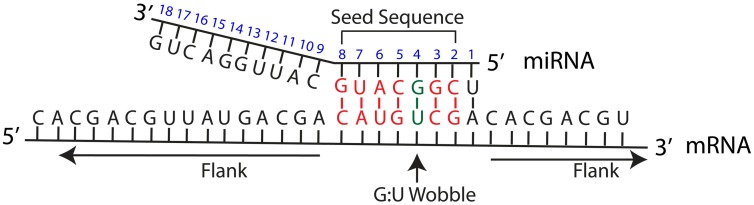
\includegraphics[scale=3]{results/seedmatching.png} 
\caption{Scheme of seed matching}
\label{seed}
\end{figure}


\begin{figure}
\centering
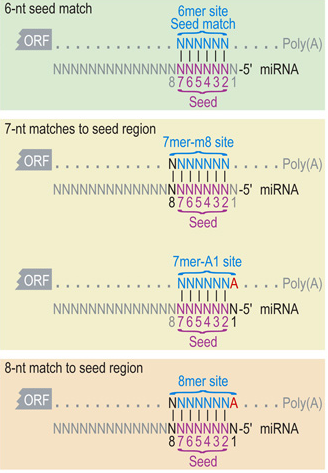
\includegraphics[scale=2.3]{results/canonical_sites.png}
\caption{Canonical sites of seed region}
\label{Fig:canonical}
\end{figure}


\begin{figure}
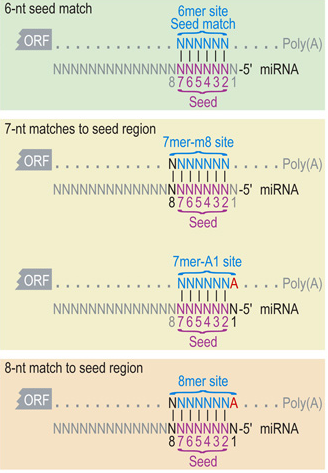
\includegraphics[scale=1]{results/canonical_sites.png}
\caption{Effectiveness of different sites}
\label{types}
\end{figure}

\subsubsection{Free energy}
The free energy of a system determines its stability and tightness of binding. If the free energy is lower than the binding between the miRNA and the mRNA sequence is tighter resulting in more evidence that this miRNA targets this mRNA. If the energy is high then the binding is not very favourable meaning the miRNA not favours to target this mRNA at this position. Some tools like RNAhybrid (Rehmsmeier et al., 2004) rely mainly on this feature. (thermodynamics von miranda)
 
\subsubsection{Conservation}
Another feature to take into account is the evolutionary conservation. If a sequence occurs across species it is defined as conserved. This implicates that this part has been maintained by evolution because of a selected function (Peterson et al., 2014). Conservation near the miRNA binding site can indicate that this part of the sequence is necessary for some mechanisms. This includes convercation of the miRNA itself as well as the conservation of the respective site of the mRNA. These conservations can be analysed with phylogentic methods.


\subsubsection{Site accessibility}
Kertesz et al. (2007) investigated the importance of site accessibility for the target prediction. (http://www.nature.com/ng/journal/v39/n10/full/ng2135.html) The mRNA generally folds into a secondary structure. Therefore the miRNA can not easily bind to its target because at first interactions within the mRNA have to be broken to make the target accessible. As a result miRNA will favourably bind to regions where the mRNA is more accessible. Kertesz et al. (2007) found that if the targets form higly stem structures the repression is reduced. If sites occur in open loop structures the repression is much higher. Summing up they found that site accessibilty is not less important than seed matching. \\

Quelle: http://www.ncbi.nlm.nih.gov/pmc/articles/PMC3927079/\\

\subsubsection{Addtional Watson-Crick pairing}
http://www.ncbi.nlm.nih.gov/pmc/articles/PMC3800283/
Grimson et al. 2013
In addition to the seed matching towards the 5' end, another complementary site towards the 3' end in the miRNA is present. Grimson et al. (2003) investigated that the highest down regulation was found when the site started at position 13 and had four or five contiguous base pairings (Figure~\ref{siteregulation}). Considering again the conservation of the nucleotides they found that outside the seed region the contiguous nucleotides starting from nucleotide 12, 13 or 14 were the most conserved ones indicating / demonstrating their functional importance (Figure~\ref{conserved}. Putting the information of seed region and additional base pairing together it can be observed that if one 7mer-m8 site is present as well as a good 3' pairing that the efficacy is the highest. Even though the difference between the efficacy of the presence of one 8mer site and the one mentioned before is not very big. But the improvement of the presence of a good 3' pairing instead of a poor one is more significant.  

In between the two complementary areas there is usually a part of non pairing nucleotides where bulges and mismatches are found.

\begin{figure}
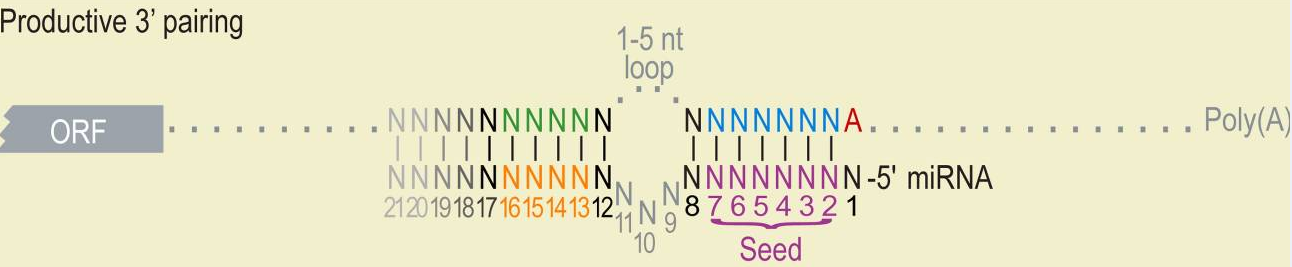
\includegraphics[scale=0.3]{results/additional_pairing.PNG}
\label{addipairing}
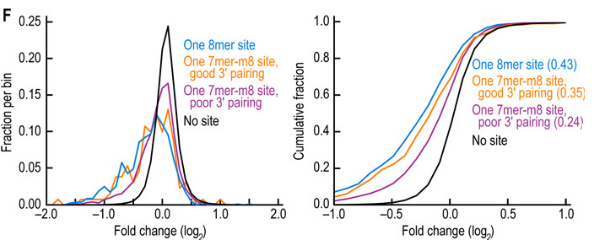
\includegraphics[scale=0.5]{results/site_efficacy.PNG} 
\label{efficacy}
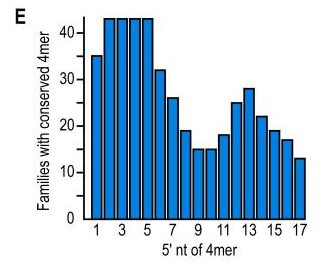
\includegraphics[scale=0.5]{results/sites_conserved.PNG} 
\label{conserved}
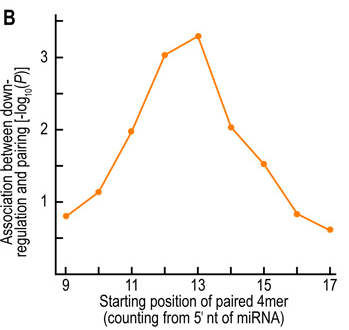
\includegraphics[scale=0.5]{results/sites_regulation.PNG} 
\label{siteregulation}
\end{figure}


\subsubsection{Other features}
To get an even more reliable and precise prediction additional features can be considered. The presence of GU-wobbles is common in targeting. In this wobble positions Guanine(G) binds to Uracil(U) even though the pairing with Cytosine would be prevalent. This special pairing is thermodynamically favourable and occurs therefore in many target interactions but results in lower repression of the translation. (http://www.ncbi.nlm.nih.gov/pmc/articles/PMC374233/) As mentioned before miRanda uses different scores for matches in their alignment step. They score the usual base pairing A-U and G-C with +5 and they penalize the other mismatches with a score of -3, excluding the pairing of G and U. This pairing is rewarded with at least +2 and therefore the GU wobbles are not penalized as much as other mismatches because they are very common. (Enright et al)
 
https://elifesciences.org/content/4/e05005

Enright et al (2005) and Doench and Sharp (2004) (http://www.ncbi.nlm.nih.gov/pmc/articles/PMC374233/)  also found that the presence of multiple miRNA target sites results in a higher repression and destabilization of the mRNA. Grimson et al (2013) (http://www.cell.com/molecular-cell/fulltext/S1097-2765(07)00407-8) further investigated that the distance between two sites is also an important criterion. Generally the repression of two present site is the multiplication of the two single once because they act independently. The interesting thing now is that if the two sites are adjacent the repression is increased and not equal to the multiplication of the single ones. The increase in repression is however not very high (Figure~\ref{sitedistance}) To investigate the effect of cooperative miRNAs they analysed a mixture of miR-1 and miR-133 and simulated three different spacings. The results show that a spacing of 4 nt did not show a cooperative repression but 6 or 8 nt spacing showed an increase in repression (Figure~\ref{sitespacing}).\\

\begin{figure}
\centering
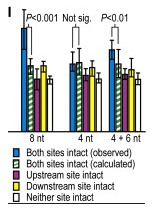
\includegraphics[scale=1.2]{results/sites_8nt.PNG}  
\caption{Cooperative repression with different site spacings}
\label{sitespacing}
\end{figure}

\begin{figure}
\centering
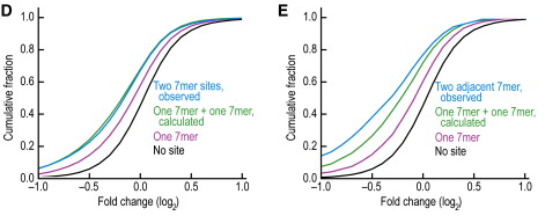
\includegraphics[scale=0.8]{results/sites_distance.PNG}
\caption{Effect of multiple sites}
\label{sitedistance}
\end{figure}

Another indicator is the position of the binding site relatively to the stop codon and the center of the UTR. Generally sites in the 3'UTR are investigated but Grimson et al. detected that sites in the Open reading frame (ORF) are slightly effective, sites in the 5'UTR not at all. Figure~\ref{siteorf} shows the different efficacies. Another characteristic concerning the site locations it the distance from the stop codon. Figure~\ref{sitestop} illustrates that in the first ~15 nt the efficacy is still very low like in the ORF but afterwards it increases much. 
The sites were present at least 15 nucleotides from the stop codon and not present in the center of long UTRs but away from it. Grimson et al. also found that the AU nucleotide content is increased in the region of conserved sites (Grimson et al., 2013).


\begin{figure}
\centering
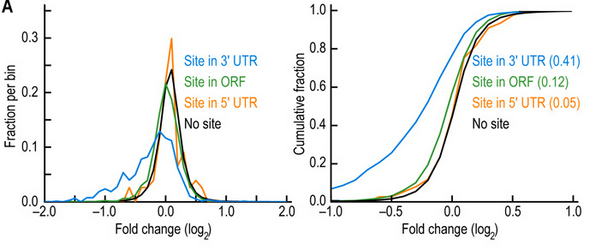
\includegraphics[scale=0.8]{results/sites_orf.PNG}
\caption{Efficacy of different site locations}
\label{siteorf}
\end{figure}

\begin{figure}
\centering
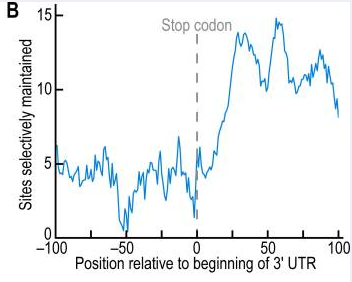
\includegraphics[scale=0.7]{results/site_stop.PNG} 
\caption{Efficacy of sites located relative to the stop codon}
\label{sitestop}
\end{figure}

   

Figure~\ref{fig:tools} shows known prediction tools and the features they consider. As mentioned above the most common feature that early all of them consider are seed matching, conservation and free energy. 


\begin{figure}
\centering
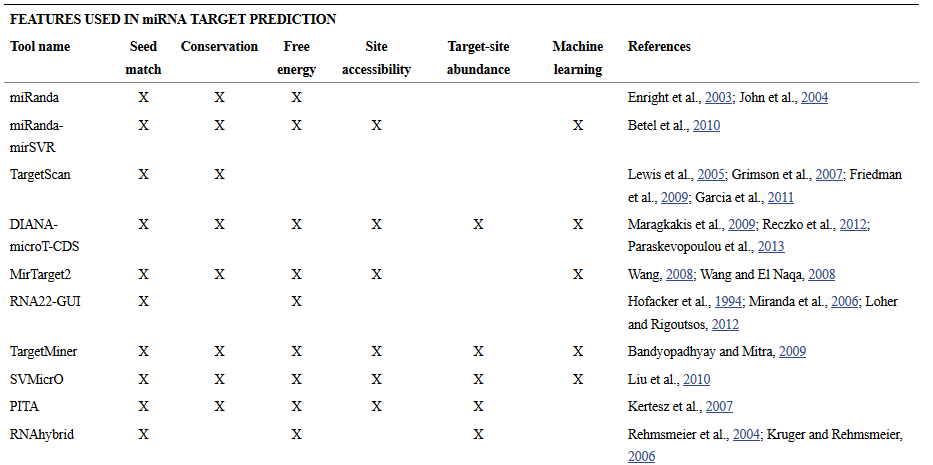
\includegraphics[scale=0.5]{results/tools.PNG}
\caption{Prediction tools and their features}
\label{fig:tools}
\end{figure}



\section{Results}
For each parameter set the alignment score for every MTI is stored in a table. Additionally the average alignment score, the standard deviation and the p-values are listed underneath. Table~\ref{table:results} shows only a summary of the table, excluding the single alignment scores. (whole table somewhere else) To draw a better comparison, the scores of the non targets are listed right under the scores of the true targets. The averages of both alignment score sets show that the scores of the true targets are in general slightly higher than the ones of the non targets. For the lower alignment scores of e.g. set 1 -2 -2 -1, resulting from really low match scores, the difference is only 0.3, so not significant. For the higher scores the difference amounts to 2. The standard deviation of the non targets is slightly higher than for the true targets but also not very significant. The p-value sheds light on whether the increase in the alignment score is significant when considering the whole set of scores. According to the listed values of the t-test this is a significant increase in the score because they are all really low. The parameters 5 -1 -8 -4 show the most significant difference with a p-value of 2.529E-61 whereas 2 -2 -5 -4 shows the least significant increase but also here the p-value is really low with 3.279E-36. So even though the average scores are not significantly different, the distribution of the score seem to be higher in the true targets than in the non targets.

\begin{table}
\label{table:results}
\footnotesize
\caption{Table of alignment results}
\vspace{0.3cm}
\begin{tabular}{c|c|c|c|c|c}
& 3 -2 -4 -4 & 5 -1 -8 -4 & 5 -2 -8 -3 & 5 -3 -8 -2 & 5 -4 -6 -4 \\
\hline\hline
Average true targets & 33.096 & 64.247 & 59.495	& 56.391 & 55.510\\
Average	non targets & 31.831 & 62.199 & 57.464 & 54.269 & 53.294 \\
\hline
Standard deviation true targets & 4.058	& 5.758 & 6.304	& 6.633 & 6.806\\
Standard deviation non targets & 4.233 & 6.510 & 6.753 & 6.876 & 7.01\\
\hline
t-test p-value & 5.934E-49 & 2.529E-61 & 1.040E-51 & 1.394E-51 & 1.744E-53 \\\hline
\end{tabular}\vspace{0.5cm}


\begin{tabular}{c|c|c|c|c}
& -4 -4 & -5 -1 & 1 -2 -2 -1 & 2 -2 -5 -4  \\
\hline\hline
Average true targets & 13.712 & 13.710 & 8.593 & 18.351\\
Average	non targets & 13.362 & 13.361 &	8.208 &	17.619 \\
\hline
Standard deviation true targets & 1.078	& 1.078	& 1.347	& 2.751\\
Standard deviation non targets & 1.311 & 1.309 & 1.385 & 2.868\\
\hline
t-test p-value & 8.824E-50 & 1.131E-49 & 8.157E-42 & 3.279E-36 \\
\hline
\end{tabular}

\end{table}

This increase in the alignment score can be also be observed when considering the distribution of the scores within the two groups of case and control. For two parameter sets such a distribution was plotted which is shown in Figure~\ref{fig:distribution}. On the x-axis the different scores are shown and on the y-axis the percentage of how many of the true targets had these scores. It can be observed that towards the higher alignment scores the percentage of true targets with this score increases. Although there are some scores that are exceptions because more non targets produced this scores than true targets. Assuming the score as the only prediction feature, the high score would classify this target as a true target. This causes therefore still many false positives. But in general the higher the score the higher the likelihood to observe a true target.

For every parameter set the complementarity of the alignments of the miRNA and gene sequence were also plotted. These are shown in Figure~\ref{fig:plot1} to Figure~\ref{fig:plot9}.

\begin{figure}
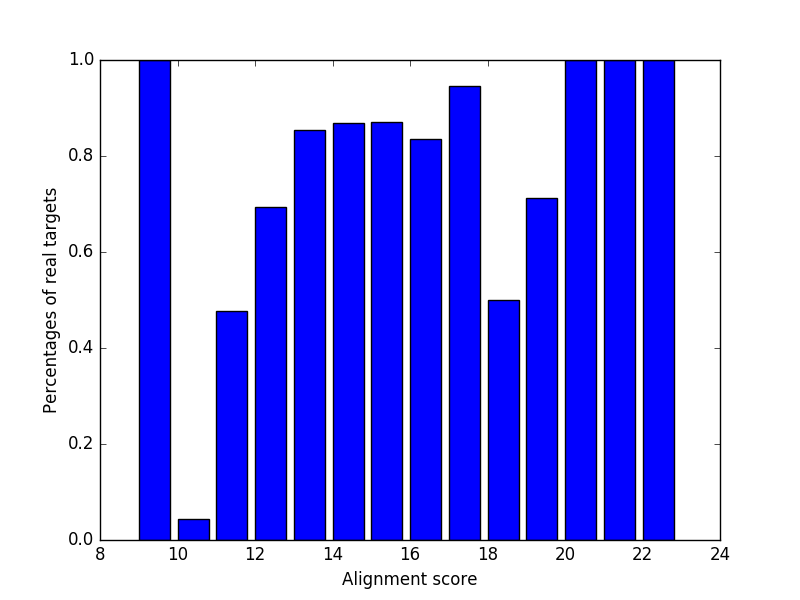
\includegraphics[scale=0.35]{results/plot_scores-4-4.png}
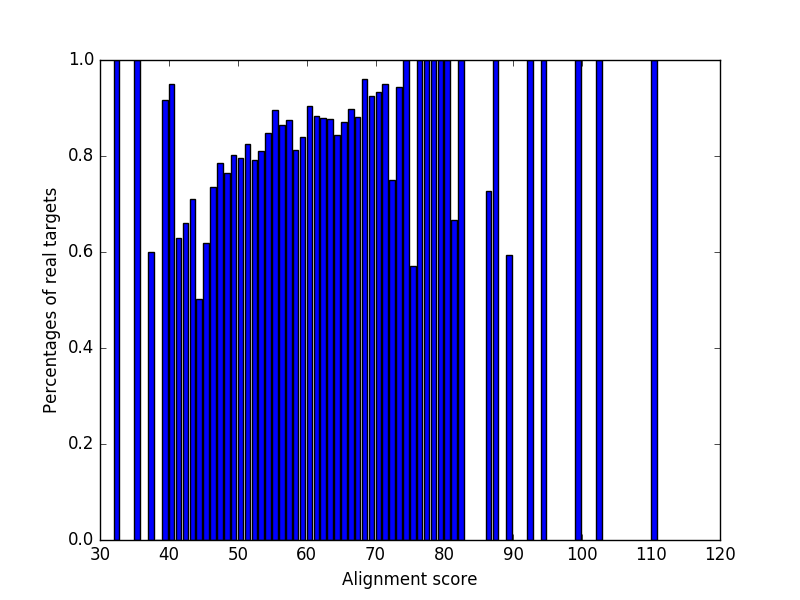
\includegraphics[scale=0.35]{results/plot_scores5-3-8-2.png}
\caption{Distribution of alignment scores, parameters -4 -4 and 5 -3 -8- 2}
\label{fig:distribution}
\end{figure}

\begin{figure}
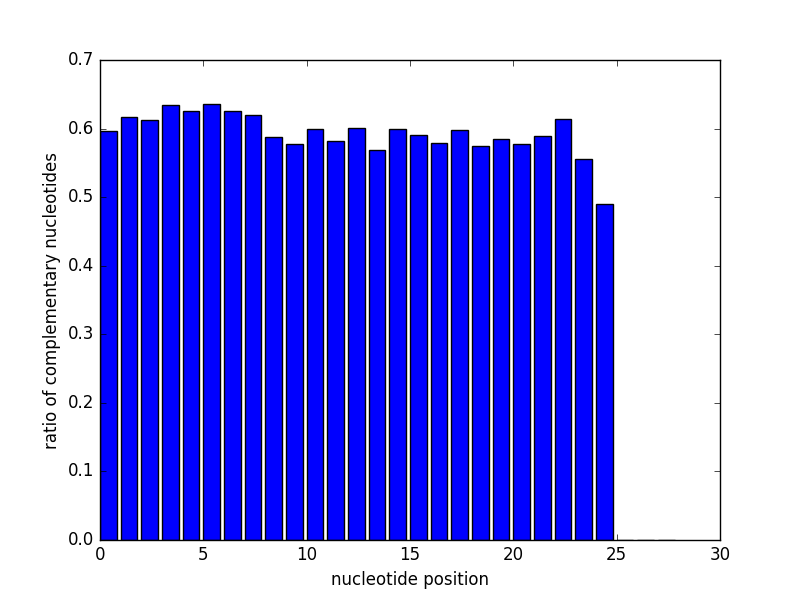
\includegraphics[scale=0.2]{results/ratio-5-1.png}
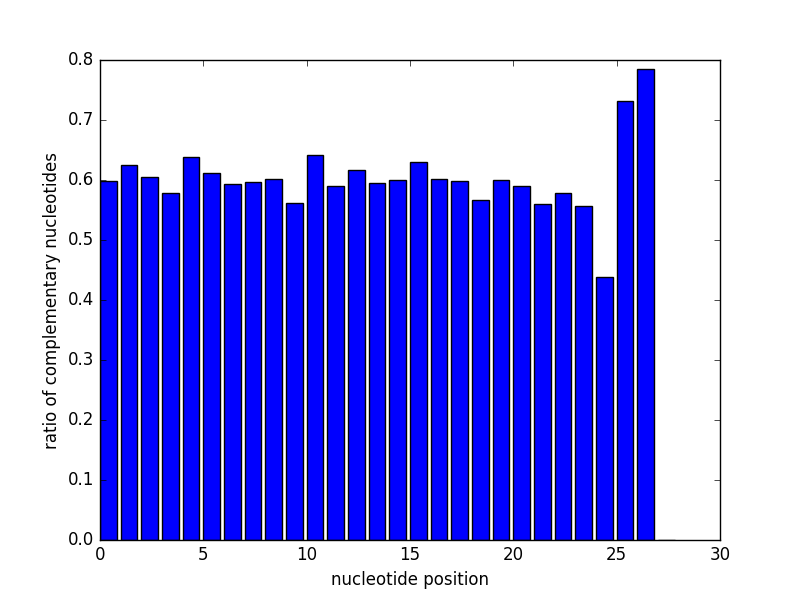
\includegraphics[scale=0.2]{results/non-ratio-5-1.png}
\caption {targets left, non targets right, parameter: -5 -1}
\label{fig:plot1}
\end{figure}

\begin{figure}
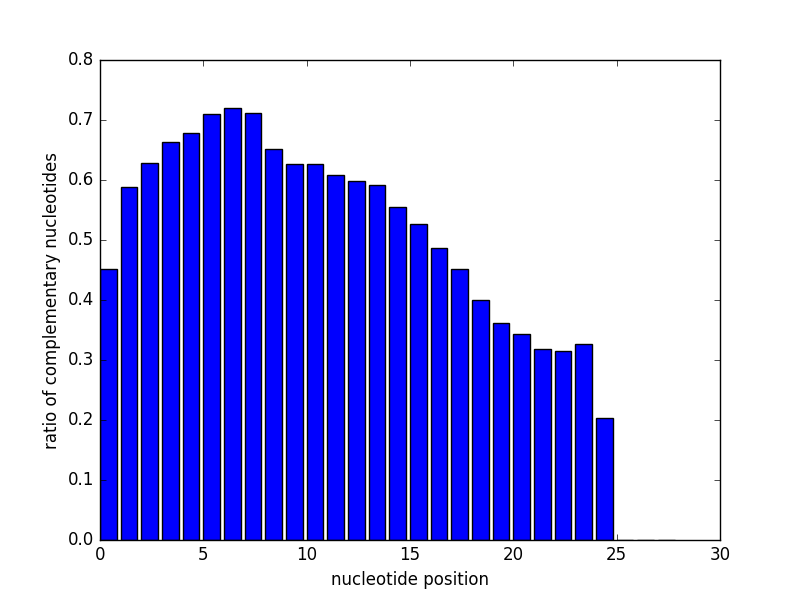
\includegraphics[scale=0.2]{results/ratio1-2-2-1.png}
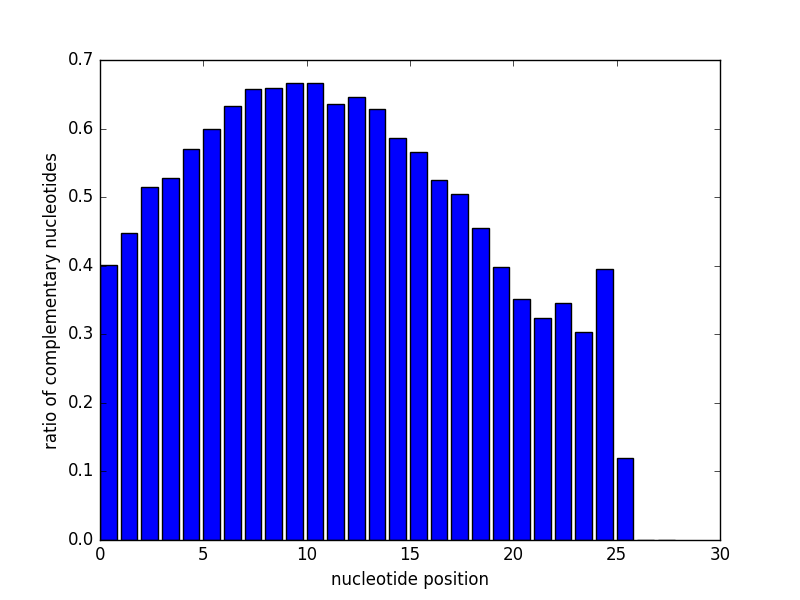
\includegraphics[scale=0.2]{results/non-ratio1-2-2-1.png}
\caption {targets left, non targets right, parameter: 1 -2 -2 -1}
\label{fig:plot2}
\end{figure}

\begin{figure}
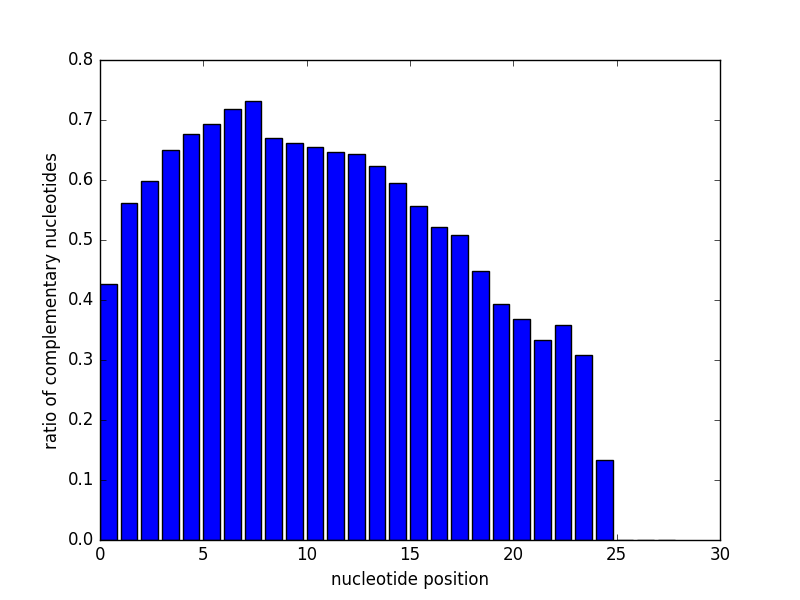
\includegraphics[scale=0.2]{results/ratio2-2-5-4.png}
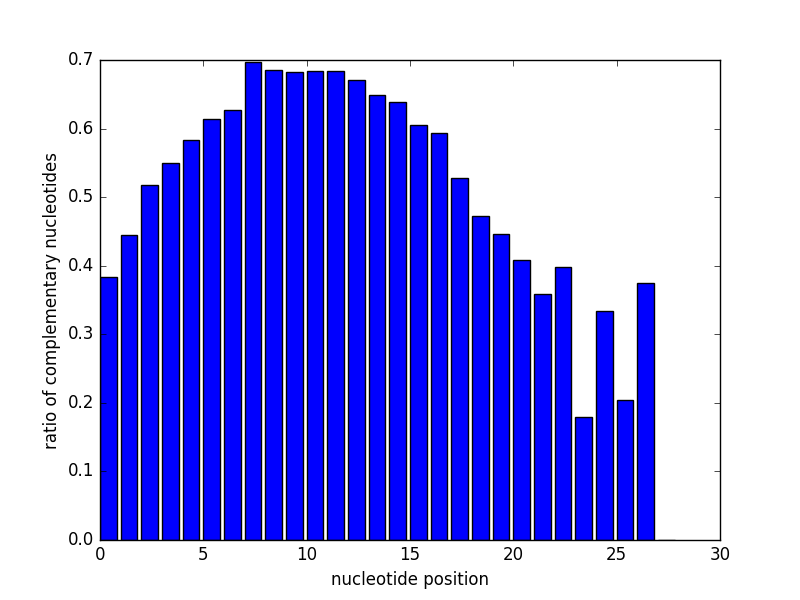
\includegraphics[scale=0.2]{results/non-ratio2-2-5-4.png}
\caption {targets left, non targets right, parameter: 2 -2 -5 -4}
\label{fig:plot3}
\end{figure}

\begin{figure}
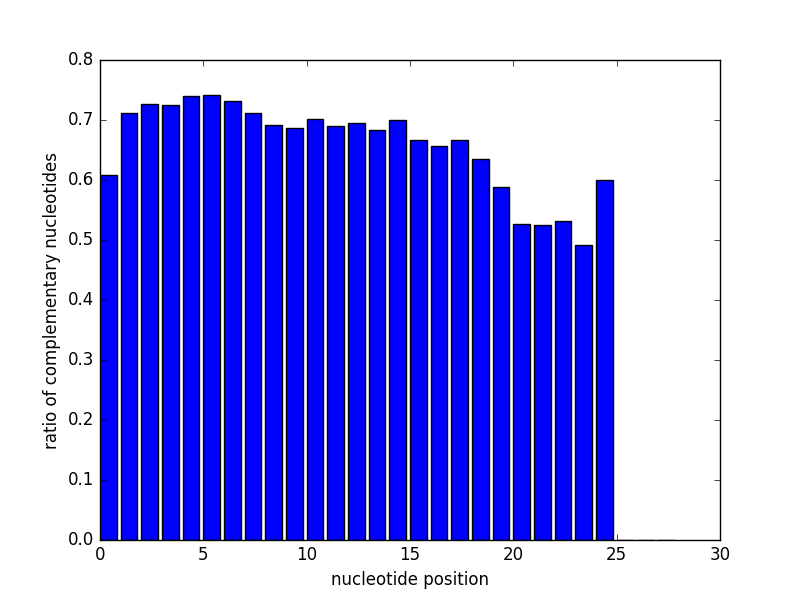
\includegraphics[scale=0.2]{results/ratio3-2-4-4.png}
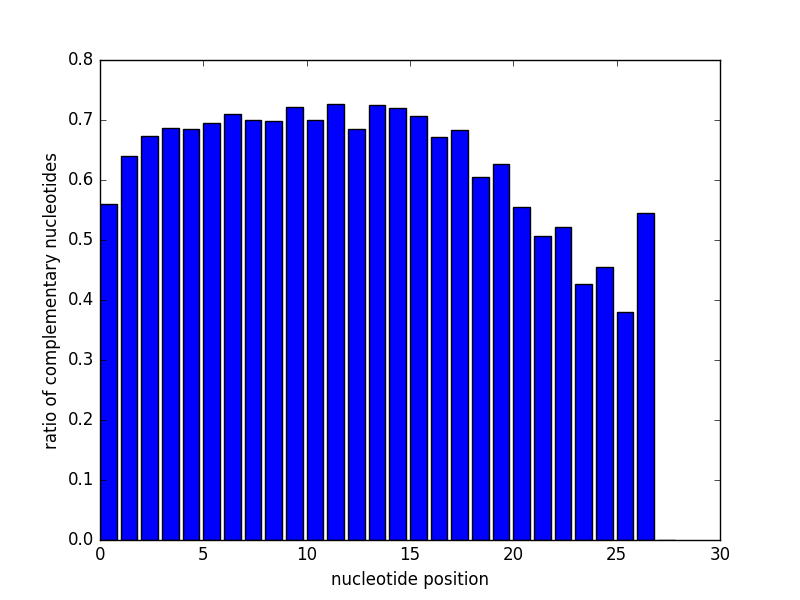
\includegraphics[scale=0.2]{results/non-ratio3-2-4-4.png}
\caption {targets left, non targets right, parameter: 3 -2 -4 -4}
\label{fig:plot4}
\end{figure}

\begin{figure}
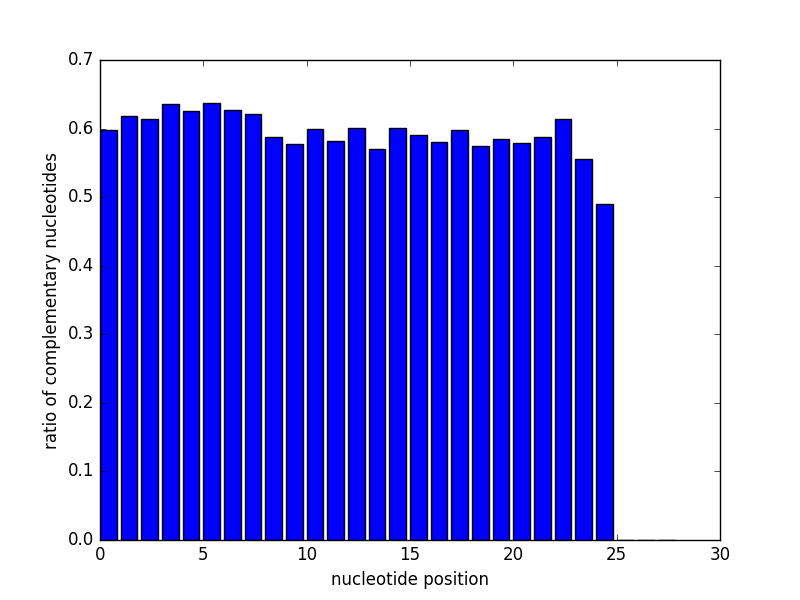
\includegraphics[scale=0.2]{results/ratio-4-4.png}
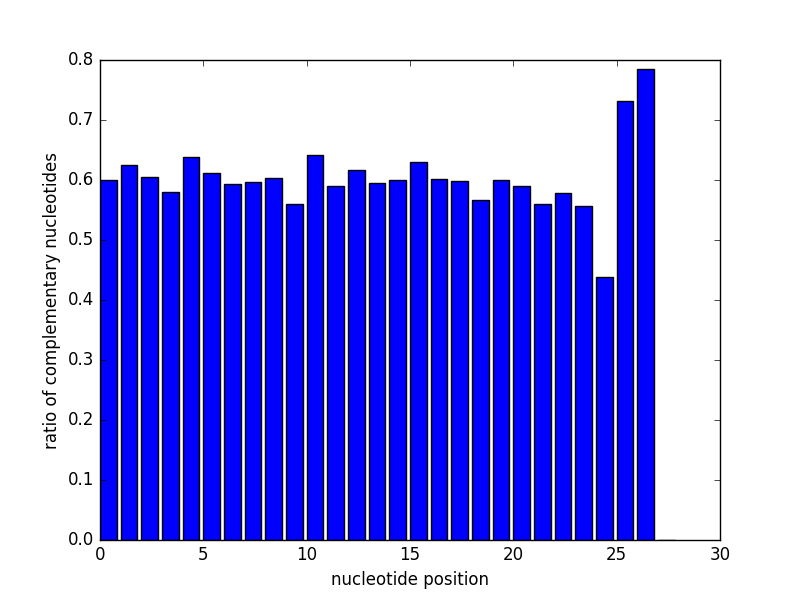
\includegraphics[scale=0.2]{results/non-ratio-4-4.png}
\caption {targets left, non targets right, parameter: -4 -4}
\label{fig:plot5}
\end{figure}

\begin{figure}
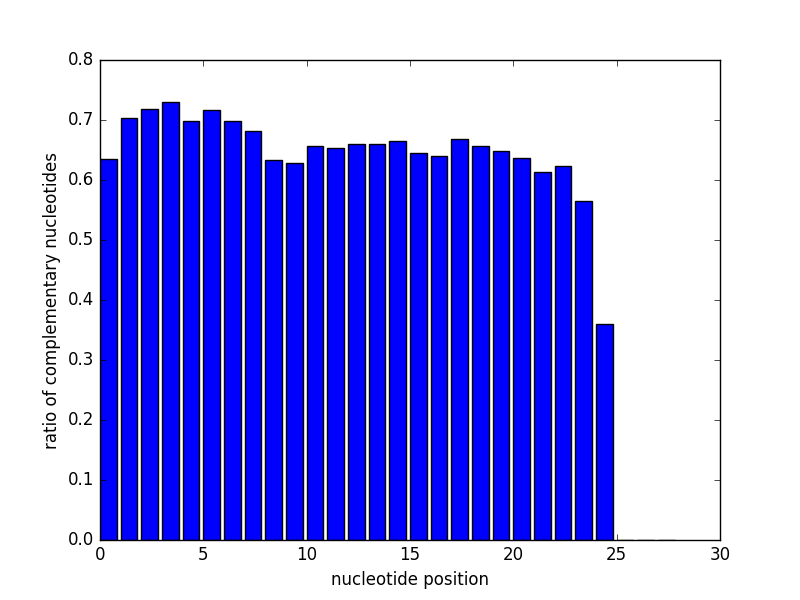
\includegraphics[scale=0.2]{results/ratio5-1-8-4.png}
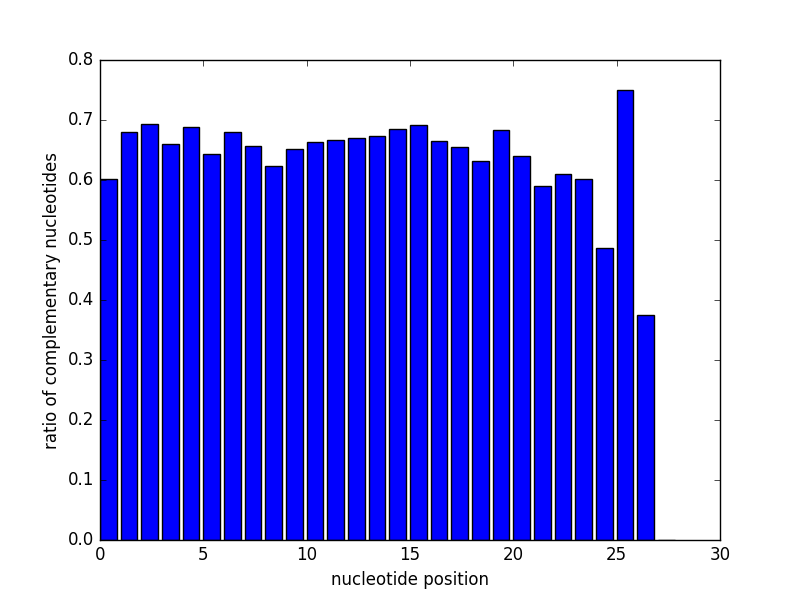
\includegraphics[scale=0.2]{results/non-ratio5-1-8-4.png}
\caption {targets left, non targets right, parameter: 5 -1 -8 -4}
\label{fig:plot6}
\end{figure}

\begin{figure}
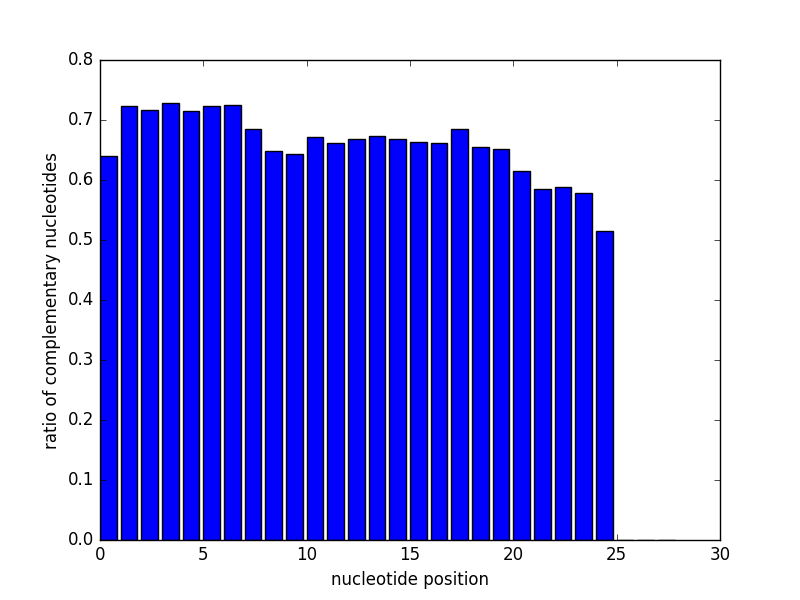
\includegraphics[scale=0.2]{results/ratio5-2-8-3.png}
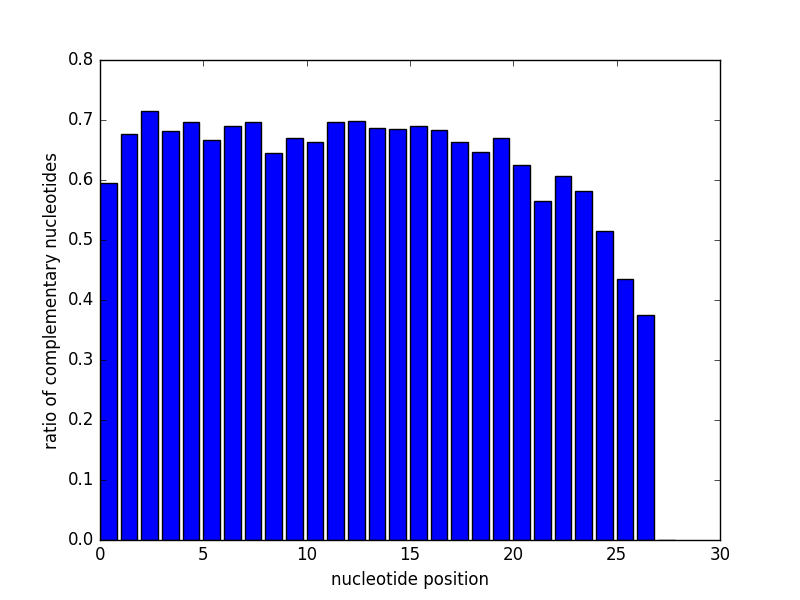
\includegraphics[scale=0.2]{results/non-ratio5-2-8-3.png}
\caption {targets left, non targets right, parameter: 5 -2 -8 -3}
\label{fig:plot7}
\end{figure} 

\begin{figure}
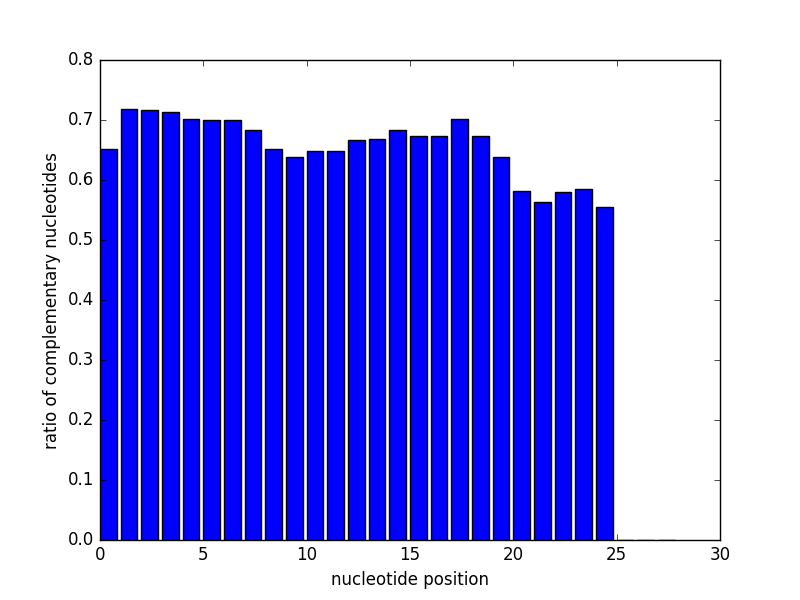
\includegraphics[scale=0.2]{results/ratio5-3-8-2.png}
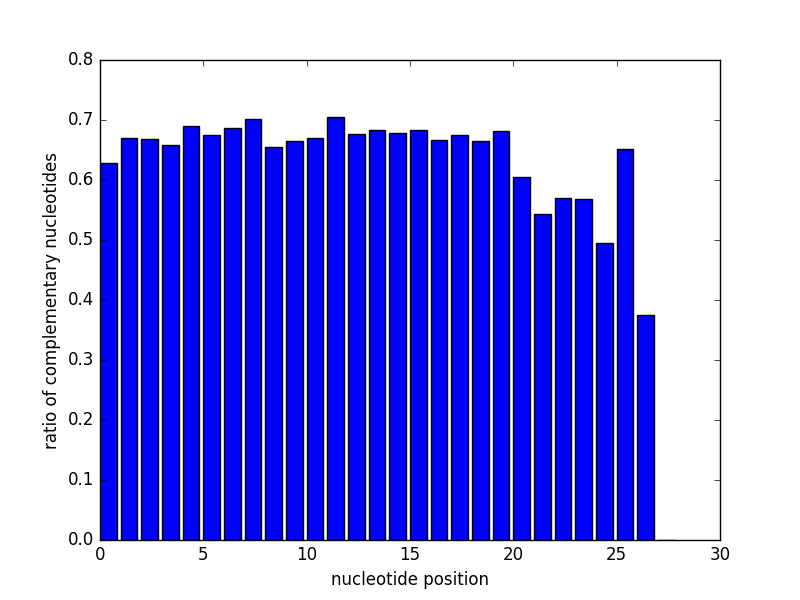
\includegraphics[scale=0.2]{results/non-ratio5-3-8-2.png}
\caption {targets left, non targets right, parameter: 5 -3 -8 -2}
\label{fig:plot8}
\end{figure}

\begin{figure}
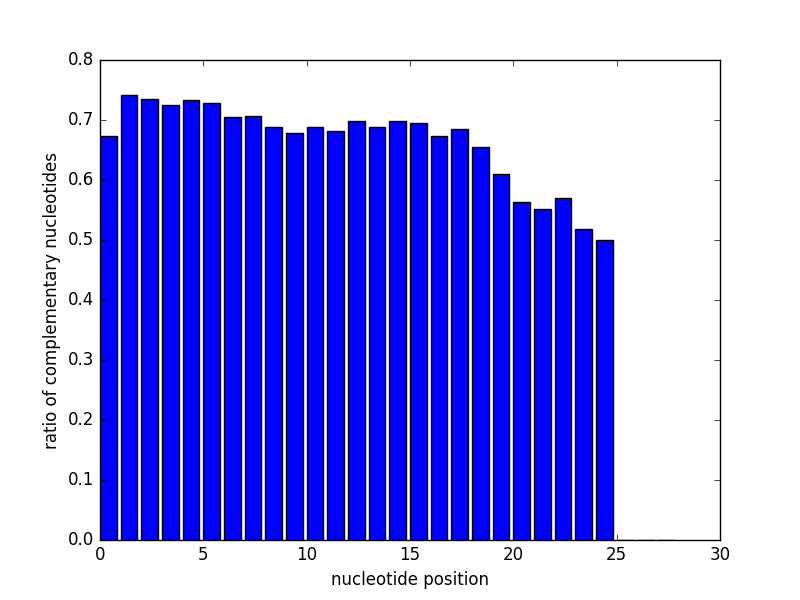
\includegraphics[scale=0.2]{results/ratio5-4-6-4.png}
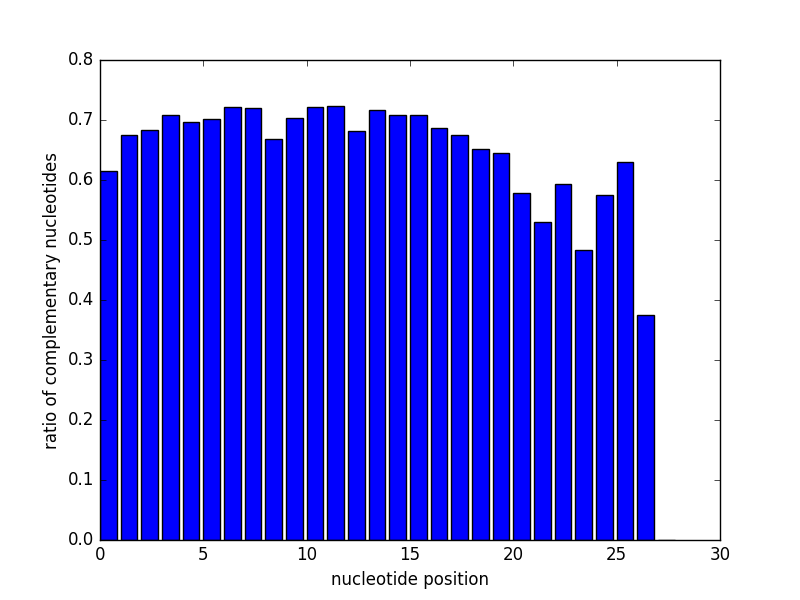
\includegraphics[scale=0.2]{results/non-ratio5-4-6-4.png}
\caption {targets left, non targets right, parameter: 5 -4 -6 -4}
\label{fig:plot9}
\end{figure}
 

The x-axis of the plots shows the positions one to 22 or more of the miRNA, the y-axis the ratio of complementary bases at this position considering all alignments produced with these parameters. For some sets there is not a significant difference between true targets and non targets, e.g. for parameters -5 -1 (Figure~\ref{fig:plot1}). Regarding set 1 -2 -2 -1 and Figure~\ref{fig:plot2} for the true target an increase in complementarity in the seed region can be observed. On the other hand the ratio towards the end gets really low down to only 30\% of the bases were complementary to the target sequence. In comparison, maximum of complementarity of the non targets is shifted towards the central positions, not showing the typical seed region. Notably the plot of the true targets does not show the complementary region towards the 3' end. Considering the other figures of the complementarities there are no significant differences between the two groups. For the non targets the complementarity is almost as high as for the true targets, gaining no reliable information for the prediction. This implicates that the consideration of the complementarities of the miRNA positions is no significant and reliable prediction feature.

The analysis of the alignment starting positions were not really successful. Table~\ref{tab:positions} shows the number of the own predicted positions that were also given in the miRTarBase. It can be seen that two sets deliver only half the number of the other. These two sets also use very similar parameters. This shows that the alignment positions strongly depend on the selected parameters. In comparison to the given number of about 3700 provided positions in the miRTarBase the numbers of the respective own found ones are in general not very high. This can be due to the different sizes of the UTRs of the genes. In this research they are from the UCSC website whereas the miRTarBase may use another source. Therefore the sizes can be a bit different. To eliminate these small disagreements I allowed a window of 10 positions where the starting position can be. So if the provided miRTarBase position is given, the own predicted position is classified as consistent if the position lies in a window of +5 or -5 related to the miRTarBase position. 


\begin{table}
\label{tab:positions}
\caption{Number of common alignment starting positions}
\vspace{0.3cm}
\begin{tabular}{c||c|c|c|c|c} 
& 3 -2 -4 -4 & 5 -1 -8 -4 & 5 -2 -8 -3 & 5 -3 -8 -2 & 5 -4 -6 -4  \\
\hline\hline
Found number & 815 & 804 & 388 & 411 & 800\\
\hline
\end{tabular}
\vspace{0.5cm}

\begin{tabular}{c||c|c|c|c}
& 1 -2 -2 -1 & 2 -2 -5 -4 & -4 -4 & -5 -1 \\
\hline\hline
Found number & 882 & 793 & 776 & 845  \\
\hline
\end{tabular}
\end{table}





\end{document}